\usetikzlibrary{shadings,shadows,shapes.arrows}

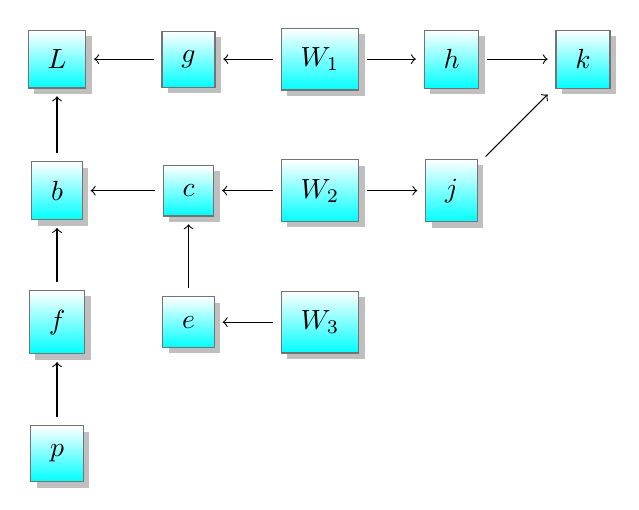
\begin{tikzpicture}
	\tikzstyle{blockstyle} = [draw,drop shadow,outer sep=3,inner sep=7,line width=1, thin, draw=black!55,
							top color=white,bottom color=cyan,align=center]	
								
	\begin{scope}[scale=1.67]
		\node[blockstyle] (L) at (0,0) {$L$};
		\node[blockstyle] (g) at (1,0) {$g$};
		\node[blockstyle] (W1) at (2,0) {$W_1$};
		\node[blockstyle] (h) at (3,0) {$h$};
		\node[blockstyle] (k) at (4,0) {$k$};
		\node[blockstyle] (b) at (0,-1) {$b$};
		\node[blockstyle] (c) at (1,-1) {$c$};
		\node[blockstyle] (W2) at (2,-1) {$W_2$};
		\node[blockstyle] (j) at (3,-1) {$j$};
		\node[blockstyle] (f) at (0,-2) {$f$};
		\node[blockstyle] (e) at (1,-2) {$e$};
		\node[blockstyle] (W3) at (2,-2) {$W_3$};
		\node[blockstyle] (p) at (0,-3) {$p$};
	\end{scope}
	
	\draw[<-] (L) -- (g);
	\draw[<-] (g) -- (W1);
	\draw[->] (W1) -- (h);
	\draw[->] (h) -- (k);
	\draw[->] (b) -- (L);
	\draw[<-] (b) -- (c);
	\draw[<-] (c) -- (W2);
	\draw[->] (W2) -- (j);
	\draw[->] (j) -- (k);
	\draw[->] (f) -- (b);
	\draw[->] (p) -- (f);
	\draw[->] (e) -- (c);
	\draw[<-] (e) -- (W3);

\end{tikzpicture}